
%% ****** Start of file template.aps ****** %
%%
%%
%%   This file is part of the APS files in the REVTeX 4 distribution.
%%   Version 4.0 of REVTeX, August 2001
%%
%%
%%   Copyright (c) 2001 The American Physical Society.
%%
%%   See the REVTeX 4 README file for restrictions and more information.
%%
%
% This is a template for producing manuscripts for use with REVTEX 4.0
% Copy this file to another name and then work on that file.
% That way, you always have this original template file to use.
%
% Group addresses by affiliation; use superscriptaddress for long
% author lists, or if there are many overlapping affiliations.
% For Phys. Rev. appearance, change preprint to twocolumn.
% Choose pra, prb, prc, prd, pre, prl, prstab, or rmp for journal
%  Add 'draft' option to mark overfull boxes with black boxes
%  Add 'showpacs' option to make PACS codes appear
%  Add 'showkeys' option to make keywords appear

\documentclass{cmspaper}

\usepackage{graphicx}
\usepackage{subfigure}
%\documentclass[aps,prl,preprint,superscriptaddress]{revtex4}
%\documentclass[aps,prd,twocolumn,superscriptaddress]{revtex4}

% You should use BibTeX and apsrev.bst for references
% Choosing a journal automatically selects the correct APS
% BibTeX style file (bst file), so only uncomment the line
% below if necessary.
%\bibliographystyle{apsrev}
\newcommand{\met}{\mbox{$E_T\hspace{-1.1em}/$\hspace{0.7em}}}


\begin{document}

% Use the \preprint command to place your local institutional report
% number in the upper righthand corner of the title page in preprint mode.
% Multiple \preprint commands are allowed.
% Use the 'preprintnumbers' class option to override journal defaults
% to display numbers if necessary
%\preprint{}


%Title of paper
\title{Search for Higgs boson in $WW \rightarrow l^{+}l^{-}\nu\nu$ using Matrix Element base discriminant.}


% repeat the \author .. \affiliation  etc. as needed
% \email, \thanks, \homepage, \altaffiliation all apply to the current
% author. Explanatory text should go in the []'s, actual e-mail
% address or url should go in the {}'s for \email and \homepage.
% Please use the appropriate macro foreach each type of information

% \affiliation command applies to all authors since the last
% \affiliation command. The \affiliation command should follow the
% other information
% \affiliation can be followed by \email, \homepage, \thanks as well.
\author{All of us}
%\email[]{Your e-mail address}
%\homepage[]{Your web page}
%\thanks{}
%\altaffiliation{}


%Collaboration name if desired (requires use of superscriptaddress
%option in \documentclass). \noaffiliation is required (may also be
%used with the \author command).
%\collaboration can be followed by \email, \homepage, \thanks as well.
%\collaboration{}
%\noaffiliation

\date{\today}

\begin{abstract}
In this note we present a search for Standard Model Higgs boson in the $WW \rightarrow l^{+}l^{-}\nu\nu$ final state 
using Matrix Element based discriminant. We search for the Higgs boson in XXX $pb^{-1}$ of $pp$ collision data at
$\sqrt{s}=7$ TeV. Events are required to have two reconstructed leptons, muons or electrons, and no reconstructed jets.
We compare performance of the Matrix Element method to the cut-based and Boosted Decision Tree based analyses. 
Signal and background yields are extrapolated to data correspoding to integrated luminosity of 1 fb$^{-1}$. 
\end{abstract}

% insert suggested PACS numbers in braces on next line
% insert suggested keywords - APS authors don't need to do this
%\keywords{}

\maketitle

% body of paper here - Use proper section commands
% References should be done using the \cite, \ref, and \label commands

\section{Introduction}
 The Standard Model (SM) of elementary particles describes a universe in which fermions, the fundamental constituents of 
matter, interact via fundamental forces propagated by gauge bosons. This description of elementary particles and their 
interactions has been validated extensively through precision experiments and found to be incredibly successful at 
describing particle physics world. However, experimentally, there remains a missing piece of the puzzle yet to be observed. 
The SM incorporates a mechanism for symmetry breaking known as the Higgs mechanism which naturally predicts the massive 
W and Z bosons as propagators of the weak force and provides a mechanism through which leptons and quarks are also 
able to acquire mass. An additional consequence of the Higgs mechanism is the existence of an associated massive scalar 
boson known as the Higgs boson, which survives as the only unobserved particle within the SM framework. 
Because of the central role of the Higgs mechanism in the SM, the discovery (or non-discovery) of the Higgs boson 
along with additional studies of its properties will either confirm the current model or point toward expected new physics 
processes at the TeV energy scale.

The SM postulates the existance of Higgs boson, but does predict its mass, which is free parameter in the model. However, experimental
measurements provide constraints on the Higgs mass. Indirect measurements of electroweak parameters indicate that the Higgs boson mass 
should be fairly low, smaller that XXX GeV at 95$\%$ confidence level. This constraints are mostly driven by measurements of 
top quank and $W$ boson mass. Moreover, direct searches at LEP excluded Higgs boson with mass below $114.4$ GeV at 95$\%$ confidence 
level. Therefore, probing mass range between 115 and 200 GeV is crucial for the Higgs boson searches.

Regardless of the mass, the dominant production of the Higgs boson is gluon fusion (GF), where Higgs is produced from a pair of 
gluons via quark (primarily top-quark) loop. Another production mechanism is the vector boson fusion (VBF) where Higgs boson
is produced from a pair of $W$ or $Z$ bosons. The relative contribution of GF and VBF to the total Higgs boson production rate
depends on the mass, but is approximately 90$\%$-10$\%$ over the range allowed by electroweak constraints. Higgs boson can be also 
produced via associated production and top-quark fusion, however contribution from these processes in the range of interest is very small.

Higgs decay is mostly driven by its mass. While di-photon decay channel dominates at low masses, searches in this channel face  
complications arising from large backgrounds and require excellent understanding of the electromagnetic calorimeter response. 
$WW \rightarrow l^{+}l^{-}\nu\nu$ final state, on the other hand, has clean signature easy to trigger on, and provides opportunity of observing
Higgs signal in a wide range of masses between 120 and 300 GeV. With large signal yield, this final state is the mot promising
discovery channel with small datasets of early CMS data. 

The main backgrounds in the $H \rightarrow WW \rightarrow l^{+}l^{-}\nu\nu$ search are diboson production, top-pair and single-top production,
$W+$jet production where hadronic jet fakes signature of a lepton, $W+\gamma$ where photon converts and produces a pair of electrons, one
of which is not-reconstructed, and Drell-Yan process.

In this note we present a search for Standard Model Higgs boson in the $WW \rightarrow ll\nu\nu$ final state 
using Matrix Element (ME) based discriminant. Triggers, event pre-selection, and reconstruction of high level objects are described 
in details in note XXX. Here, we introduce ME technique, describe its technical implemenation, summarize the event selection, 
present results and compare them to the ones obtained with cut-based and Boosted Decision Tree based approaches.

\section{Method Overview}
Kinematic properties of Higgs boson events tend to be different from these produced in background processes. Namely, due to spin correlations,
Higgs events produced via gluon fusion tend to have small angular separation between leptons with large missing transverse energy recoiling
against the di-lepton pair. Background events typically have significantly larger dilepton angular separation.  Moreover, 
transverse momenta of leptons produced in Higgs decays tend to be smaller than for most of the backgrounds. As a consequence of this,
dilepton invariant mass is on average smaller for Higgs events than for $q\bar{q} \rightarrow WW$ events, which dominate the background.

While cut-based approach attempts to find an optimal set of lepton $p_{T}$, lepton pair azimuthal separation $\phi_{ll}$, 
di-lepton invariant mass  $M_{ll}$ and \met requirements, it is beneficial to use all information about event kinematics in a correlated way. 
In other words, if $\phi_{ll}$ of an event is Higgs-like for certain $M_{H}$ hypothesis, then other parameters, such as for example 
\met, should be consistent with this hypothesis too. By building a multivariate discriminant, which explores full event kinematics in a 
correlated way, one can achieve better signal versus background separation than standard cut-based approach and, 
therefore, improve analysis sensitivity to Standard Model Higgs boson signal.

One way to create such discriminant is by employing Matrix Element method. This method has been previously used in precision measurements of 
top quark mass and cross sections, as well as searches for single top and Higgs boson production at the Tevatron.

In this method we calculate the probability for each 
recorded event to originate from a specific physics process. This is done by comparing the measured kinematic observables with the predicted 
differencial cross-section given by a Matrix Element calculation, as a function of those observables for the signal and background processes.
The discriminating power arises because the differential cross sections for signal and background events are largest in different regions
of the available phase space. The principal difference between the ME technique and other multivariate approaches (Artificial Neural Networks,
 Boosted Decision Trees, etc) is that the final discriminant is based on the results of physics calculations rather than various statistical
 methods used to solve regression problem. It is free of potential ``over-training'' dangers and can be tested on processes other than Higgs,
with larger cross-sections. However, it does have its own complication - theoretical Matrix Element calculations are performed at the 
parton level, while we reconstruct events at the detector level. Therefore, to achieve better discrimination, it is necessary to implement
transfer functions as well as detector resolution functions for reconstructed objects in the ME-based discriminant.

\section{Event Probability}
\subsection{General Considerations}
The Matrix Element method relies on evaluation of the event probability densities for the signal and background processes based on the 
Standard Model differential cross-section calculation. 

In general, a differential cross-section is given by:
\begin{equation}
d\sigma=\frac{(2\pi)^{4} \left| M \right|^{2}}{4\sqrt{(q_{1}q_{2})^{2}-m_{q_{1}}^{2}m_{q_{2}}^{2}}}d\Phi_{n}(q_{1}+q_{2};p_{1},...p_{n}),
\label{eqn:DiffXsecGeneral}  
\end{equation}
where $\left| M \right|$ is the Lorentz invariant matrix element; $q_{1}$,$q_{2}$ and $m_{q_{1}}$,$m_{q_{2}}$ are the four momenta and masses
of the incident particles (in our case quarks or gluons), and $d\Phi_{n}$ is the $n$-body phase space given by:
\begin{equation}
d\Phi_{n}(q_{1}+q_{2};p_{1},...p_{n})=\delta^{4}(q_{1}+q_{2}-\sum_{i=1}^{n}{p_{i}})\prod\frac{d^{3}p_{i}}{(2\pi)^{3}2E_{i}}.
\label{eqn:PhaseSpaceGeneral}  
\end{equation}
It is important to note here, that energies of the incident partons are not known and are distributed according to the parton density 
functions (PDFs). Therefore, for a certain set of observed kinematic properties $x$, one can write probability of observing it as:
\begin{equation}
P(x)=\frac{1}{\sigma}\int d\sigma(y)dq_{1}dq_{2}f(y_{1})f(y_{2})W(x;y),
\label{eqn:EvtProbGeneral}  
\end{equation}
where $y=(p_{1}...p_{n})$ is a set of parton level variables needed to describe an event, $d\sigma(y)$ is the differential cross-section 
in terms of $y$, $f(y_{1})$ and $f(y_{2})$ are the PDFs and $W(x;y)$ is a transfer function which maps parton level quantities to the reconstructed level. One can think of $W(x;y)$ as probability of observing a reconstructed event $x$ given event with parton level properties $y$. $\sigma$ is a normalization constant which is discussed separately below.

Assuming that momenta of the incident partons have no transverse component, the four vectors can be written as:
\begin{equation}
q_{1}=(0,0,\xi_{1}E_{beam},\xi_{1}E_{beam}),
q_{2}=(0,0,-\xi_{2}E_{beam},\xi_{2}E_{beam}),
\label{eqn:EvtProbGeneral2}  
\end{equation}
where $\xi_{1}$ and $\xi_{2}$ are fractions of proton energy carried by initial partons as given by PDFs, and $E_{beam}=3.5$ TeV. Assuming 
that the initial state partons are massles, we can re-write the ``flux'' term:
\begin{equation}
\frac{1}{\sqrt{(q_{1}q_{2})^{2}-m_{q_{1}}^{2}m_{q_{2}}^{2}}} \approx \frac{1}{2 E_{q_{1}}E_{q_{2}}}.
\label{eqn:flux}  
\end{equation}
Taking into account \ref{eqn:DiffXsecGeneral} and \ref{eqn:PhaseSpaceGeneral}, and considering final state with four particles,
 equation \ref{eqn:EvtProbGeneral} can be re-written as:
\begin{equation}
P(x)=\frac{1}{ \sigma}\int 2 \pi^{4} \left| M \right|^{2} \frac{f(y_{1})f(y_{2})}{(E_{q_{1}}E_{q_{2}})^{2}}W(x;y)d\Phi_{4}dE_{q_{1}}dE_{q_{2}},
\label{eqn:EvtProbGeneral2}  
\end{equation}
or
\begin{equation}
P(x)=\frac{1}{\sigma }\int 2 \pi^{4} \left| M \right|^{2} \frac{f(\xi_{1})f(\xi_{2})}{\xi_{1}\xi_{2}E_{beam}^{2}}W(x;y)d\Phi_{4}d\xi_{1}d\xi_{2},
\label{eqn:EvtProbGeneral2}  
\end{equation}

\subsection{Effect of the system boost}
Equation \ref{eqn:EvtProbGeneral2} is derived assuming no transverse component of the incident partons, which is true at the Leading Order. 
At the next-to-leading order (NLO), however, the ISR can generate create transverse momentum of the system. Distribution of the system
transverse momentum depends on the amount ISR and its $p_{T}$ spectrum, and therefore may vary for different physics processes. In the 
presense of transverse boost, the general probability expression can be written as:
\begin{equation}
P(x)=\frac{1}{\sigma }\int 2 \pi^{4} \left| M \right|^{2} \frac{f(\xi_{1})f(\xi_{2})}{\xi_{1}\xi_{2}E_{beam}^{2}}\epsilon(y)G(x;y)d\Phi_{4}d\xi_{1}d\xi_{2}K(k_{x},k_{y})dk_{x}dk_{y},
\label{eqn:EvtProbGeneralWithBoost}  
\end{equation}
where $K(k_{x},k_{y})$ is the transverse momentum distribution and $W(x;y)=\epsilon(y)G(x;y)$ is factorized into reconstruction efficiency term $\epsilon(y)$
and resolution functions $G(x,y)$ accounting for detector resolution effects. 

\subsection{Normalization Constant}
If integration is performed over the entire kinematic phase space, then the normalization term $\sigma$ is equal to the total cross-section $\sigma_{total}$. However, if integration is performed only over the acceptance region, then $\sigma=A\sigma_{total}$, where $A$ is acceptance term for a given physics process, or in other words fraction of the total cross-section falling into the acceptance region. Acceptance term $A$ can be derived as:
\begin{equation}
A=\frac{N_{accepted}}{\sigma_{total}\times L},
\label{eqn:Acceptance}  
\end{equation}
where $N_{accepted}$ is expected yield of events passing acceptance selection, and $L$ is the integrated luminosity.

\subsection{$l^{+}l^{-}\nu\nu$ final state }
For Higgs to $WW$ leptonic final state, assuming no jet activity, 
set of reconstructed quantities can be written as $x=(\vec{p}_{l1},\vec{p}_{l2}, \met_{x},  \met_{y})$.
The complication of this state is that it is not fully reconstructed, information about $z$-components of neutrino 
momenta as well as individual neutrino transverse components are missing. It is, therefore, necessary to integrate over these 
unknown quantities. Expression \ref{eqn:EvtProbGeneralWithBoost} for this case can be written as:
\begin{eqnarray}
P(x)=\frac{1}{\sigma }\int 2 \pi^{4} \left| M \right|^{2} \frac{f(\xi_{1})f(\xi_{2})}{\xi_{1}\xi_{2}E_{beam}^{2}}
\epsilon(\vec{p}_{l1})\epsilon(\vec{p}_{l1}) \times \nonumber \\ 
                         G(p_{l1},p_{l2}, \met_{x},  \met_{y}; q_{l1}, q_{l2}, p_{\nu_{1,x}}+  p_{\nu_{2,x}}, p_{\nu_{1,y}}+p_{\nu_{2,y}})d\Phi_{4}d\xi_{1}d\xi_{2} \times \nonumber \\
                         K(k_{x},k_{y})dk_{x}dk_{y}\delta(p_{\nu_{1,x}}+p_{\nu_{2,x}}-\met_{x})\delta(p_{\nu_{1,y}}+p_{\nu_{2,y}}-\met_{y}).
\label{eqn:EvtProbGeneralWithBoost2L2nu}  
\end{eqnarray}
where $q_{l1}$ and $q_{l2}$ are true momenta of the leptons.

\section{Event Selection}
The fully leptonic final state consists of two isolated leptons and large missing energy from the two undetectable neutrinos. 
The following event selection requrements have been applied:

\begin{enumerate}                                                                                                     
\item We select events that pass pre-defined lepton triggers.                                                                 
\item We then select those events with two oppositely charged high $p_{T}$ isolated leptons ($ee$, $\mu\mu$, $e\mu$) requiring:
\begin{itemize}
   \item $p_{T}>20~GeV/c$ for the leading lepton;                                                                        
   \item $p_{T}>10~GeV/c$ for the trailing lepton;                                                                            
   \item standard identification and isolation requirements on both leptons.                                                  
\end{itemize}                                                                                                                  
\item 
We apply a common preselection, which requires in brief:                                                           
\begin{itemize}                                                                                                                
\item no restriction on the number of reconstructed jets;                                                                      
\item exactly two high $p_{T}$ leptons that are inconsistent with a $Z$ boson or top quark decay;              
\item large transverse missing energy due to the neutrinos.
\end{itemize}                                                                                                                  

\item Finally, we apply $M_{H}$ dependent di-lepton invariant mass requirement which is
summarized in Table XXX.                                                                                               
\end{enumerate}             

\section{ Probability Calculations }
Matrix Element functions used in this analysis are obtained from  MCFM v5.8.  
MCFM provides both LO, and NLO cross-section calculations for 
all relevant background and Higgs processes in $pp$ collisions. In this analysis 
we use only LO Matrix Element. In the future we plan to improve our discriminant 
by getting advantage of NLO Matrix Element. PDF set used in event probability 
calculations is CTEQ 6.1M.

Construction of the most optimal discriminant would require calculation 
of event probabilities for each of the background processes. In reality, however, having 
probabilities for the signal hypothesis and primary backgrounds is sufficient for the 
desired level of discrimination. In this analysis for each event we calculate probabilities 
for gluon fusion Higgs boson production (ggH), non-resonant $qq\bar\rightarrow WW$ pair 
production (WW) and $W$+jet process where W boson is produced in association with one jet. 
For ggH we calculate event probabilities assuming 12 different Higgs mass/width
hypothesis.
                                        
\subsection{Efficiency and Transfer Functions}

Efficiency functions $\epsilon(\vec{p})$ provide probability that a lepton of certain momentum
gets reconstructed in the detector. We evaluate this probability using non-resonant $qq\bar\rightarrow WW$
separately for muons and electrons and parametrize them as a function of reconstructed level lepton $p_{T}$ and $\eta$.
The probability in each ($p_{T}$,$\eta$) bin is defines as number of fully reconstructed leptons divided 
by the number of generator level leptons. Figure~\ref{fig:lepeff_gen} shows the 
one dimensional projection of the efficiency as a function of the lepton $\eta$ and $p_{T}$. 
A scale factor to account for differences between 
data and Monte Carlo can be calculated using a tag-and-probe analysis and applied when calculating event 
probabilities for data events.

\begin{figure}[!htbp]
\begin{center}
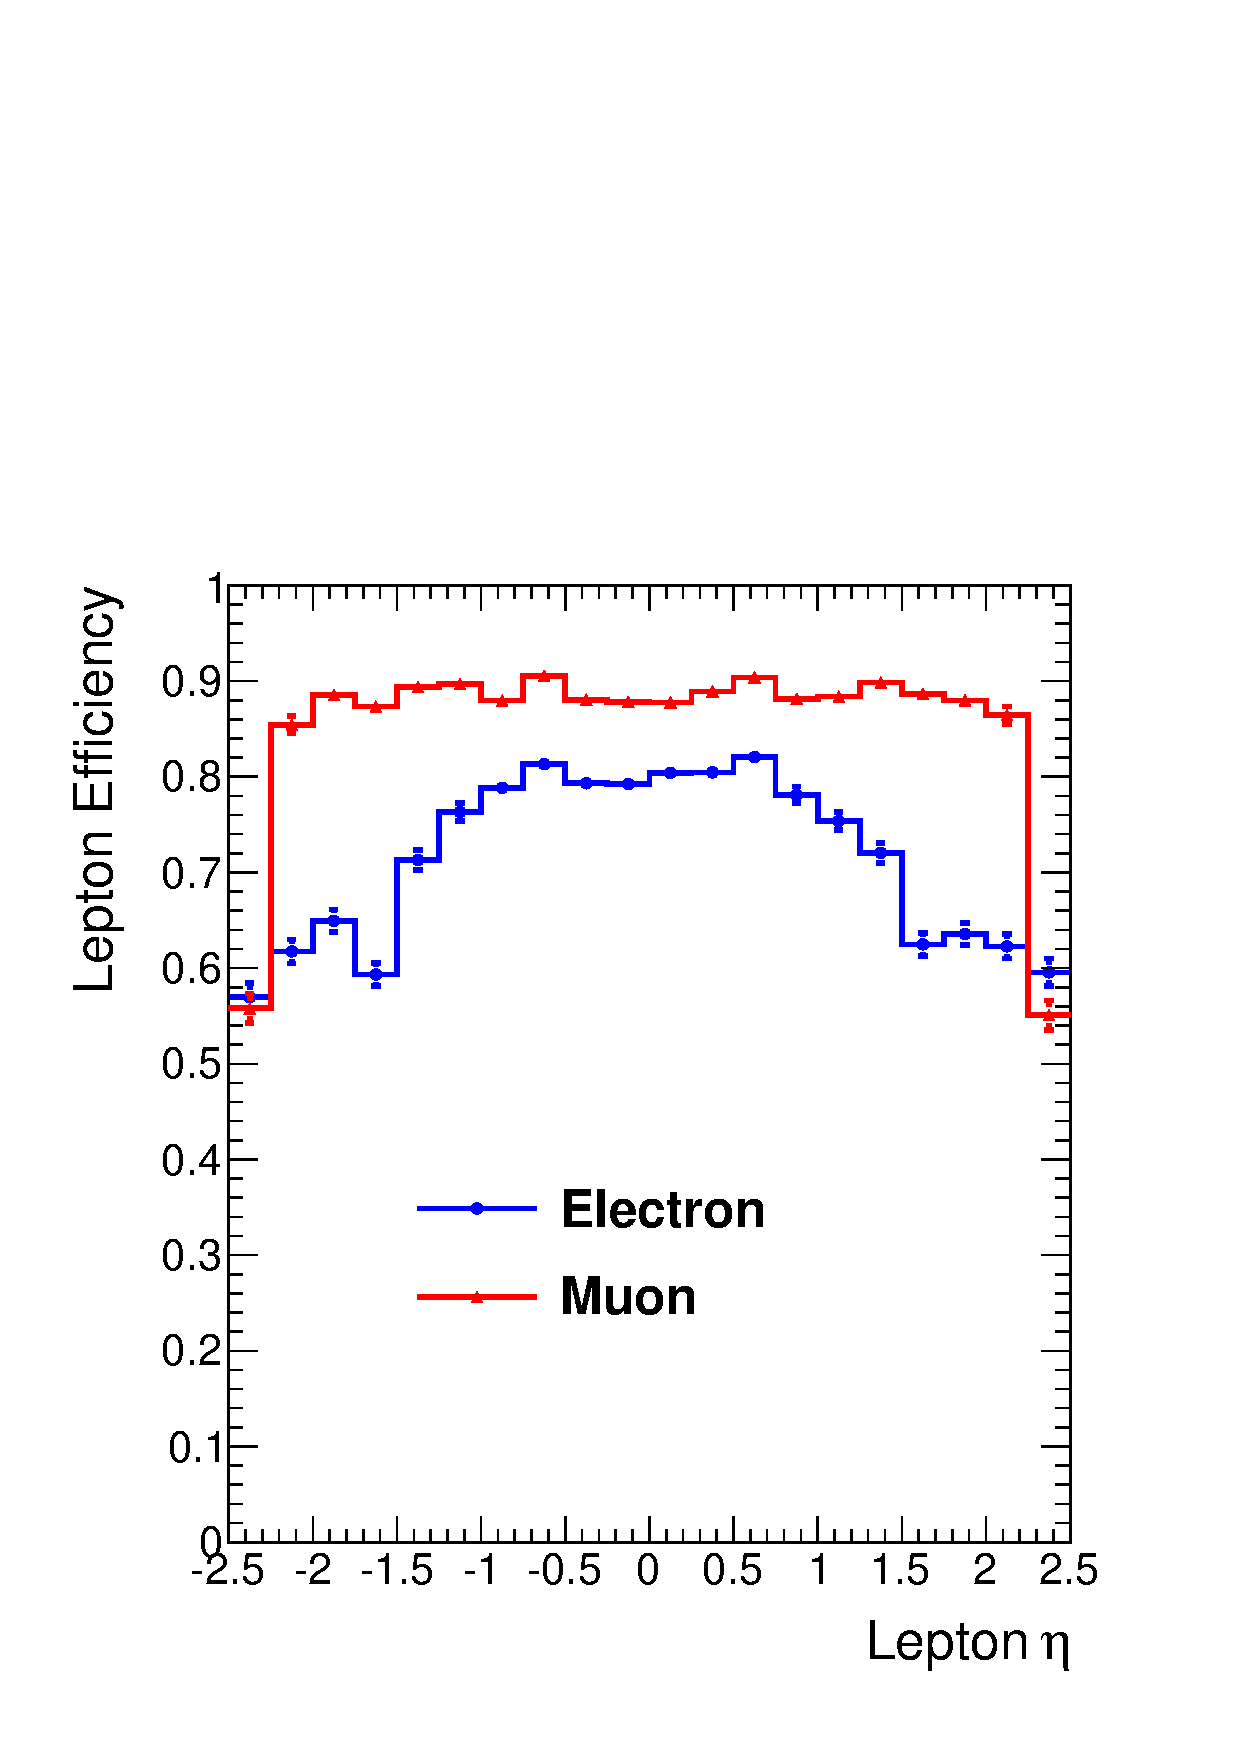
\includegraphics[width=0.4\textwidth]{figures/lepton_eff_Eta.pdf}
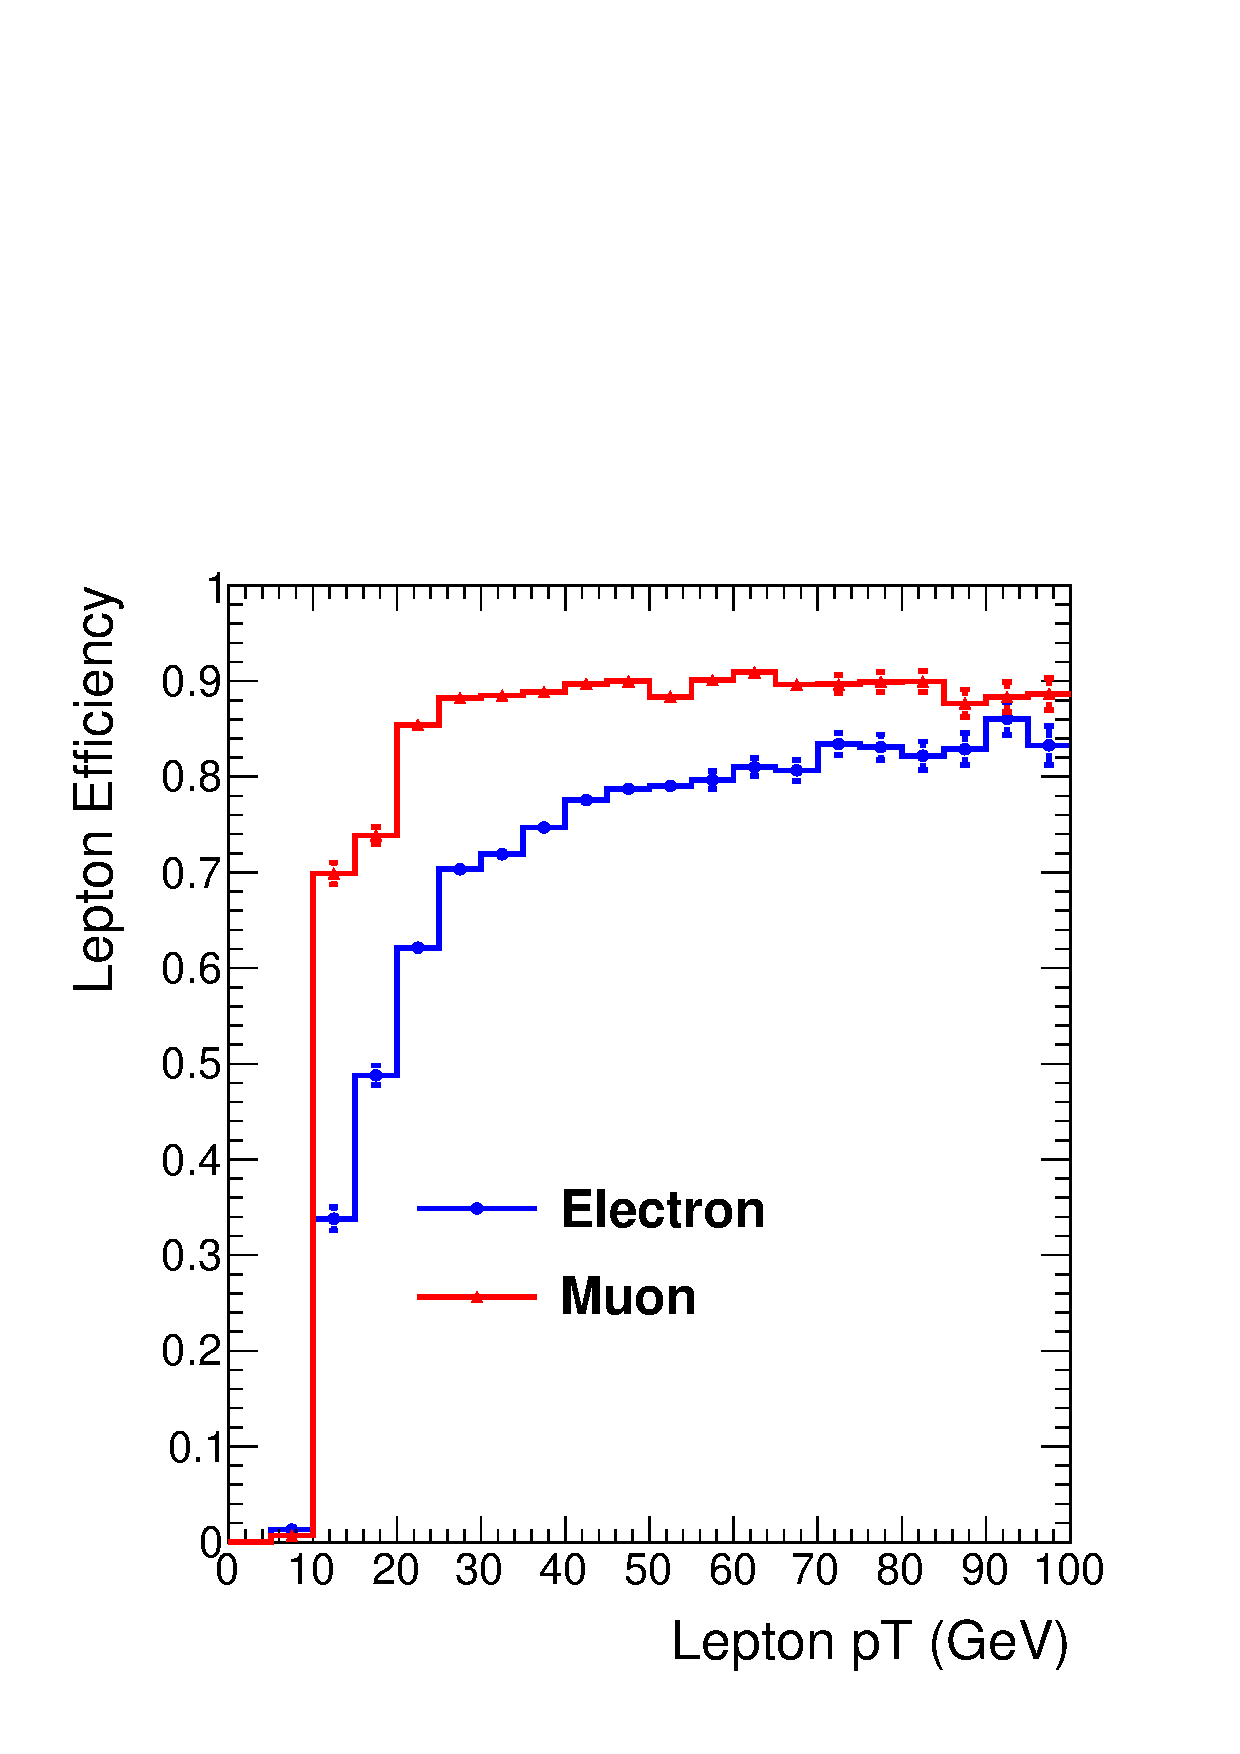
\includegraphics[width=0.4\textwidth]{figures/lepton_eff_Pt.pdf}\\
\caption{Lepton efficiency as a function of the lepton $\eta$ (left) and $p_{T}$ (right) extracted 
from the $WW$ Monte Carlo.}
\label{fig:lepeff_gen}
\end{center}
\end{figure}

Transfer functions $G(x;y)$ provide the probability of measuring the set of observable variables ($x$) originating 
from a set of production variables ($y$). The set ($y$) represents final state charged lepton and neutrino momenta at
the particle level, while the set ($x$) respresents measured lepton momenta and missing transverse energy in the CMS
detector. The general idea of these  functions is to introduce a relation between parton level objects and measured objects.
In the case of well-measured objects, such as lepton momenta, $G(x;y)$ is considered to be a $\delta$-function, I.e. the 
reconstructed lepton momenta are used in the differential cross-section calculations. For unmeasured quantities, such as
longitudinal component of neutrino momenta, the transfer function is unity. Sum of the transverse components of neutrino
momenta can be inferred from energy and momentum conservation.

Treatment of the W + jet event probability calculation deserves special discussion. For these events to be 
reconstructed in the dilepton final state, one of the reconstructed leptons has been faked by a parton 
fragmenting and hadronizing into a QCD jet which then fakes the signature of a lepton in the detector. 
To account for this effect properly, we multiply the differential cross-section for the $W$+jet process by the 
probability for a parton to be reconstructed as a lepton with the measured kinematics. This probability can be 
factorized into two terms:
\begin{eqnarray}
\begin{array}{lcl}
P(parton\rightarrow lepton)=P(parton\rightarrow FO) \times P(FO\rightarrow lepton),
\end{array} 
\end{eqnarray} 
where FO refers to a so-called ``fakeable object''. The first term in the product is measured using Monte Carlo and 
parametrized in $p_{T}$ and $\eta$. The second term is the fake rate measured in the data. The values 
of $P(parton \rightarrow lepton)$ are illustrated in Figure~\ref{fig:lepgenfr}. 

We cross check $P(parton \rightarrow lepton)$ values that we obtain using this method by comparing them to ones measured in a $\gamma$+jet 
Monte Carlo sample. We check that in both, $W$+jet and  $\gamma$+jet samples, electron fakeable objects originate 
most frequently from light quarks while muon fakeable objects are coming primarily from semi-leptonic decays of charm and bottom quarks, 
as it is shown in Figure~\ref{fig:fakeorigins}.
Then using  $\gamma$+jet events we calculate probability as ratio of the number of fakeable objects and number of jets in each $\eta$ and $p_{T}$ bin.
Probabilities obtained using these two methods agree well within the uncertainty. 

It should be also
noted that in most cases momentum of a fake lepton is significantly smaller than one of the faking parton. To account 
for this effect we use transfer function which maps parton level quark or gluon momentum into fake reconstructed lepton
momentum. We extract this function from Monte Carlo by matching status code 3 partons to fakeable objects within 
cone of $dR=0.2$. The function is parametrized in $p_{T}$ of a fakeable object and is shown in Figure~\ref{fig:ptresponse}.
In principle, not only $p_{T}$ but also direction of the parton can differ from the direction of reconstructed fakeable object.
However, we find that in vast majority of cases they lie within $dR<0.1$ (as shown in Figure~\ref{fig:partonleptondirection}) 
which has very little effect on the results of the analysis. Therefore, we do not apply any corrections to the direction
of the parton.


\begin{figure}[!htbp]                                                                                         
\begin{center}                                                                                                
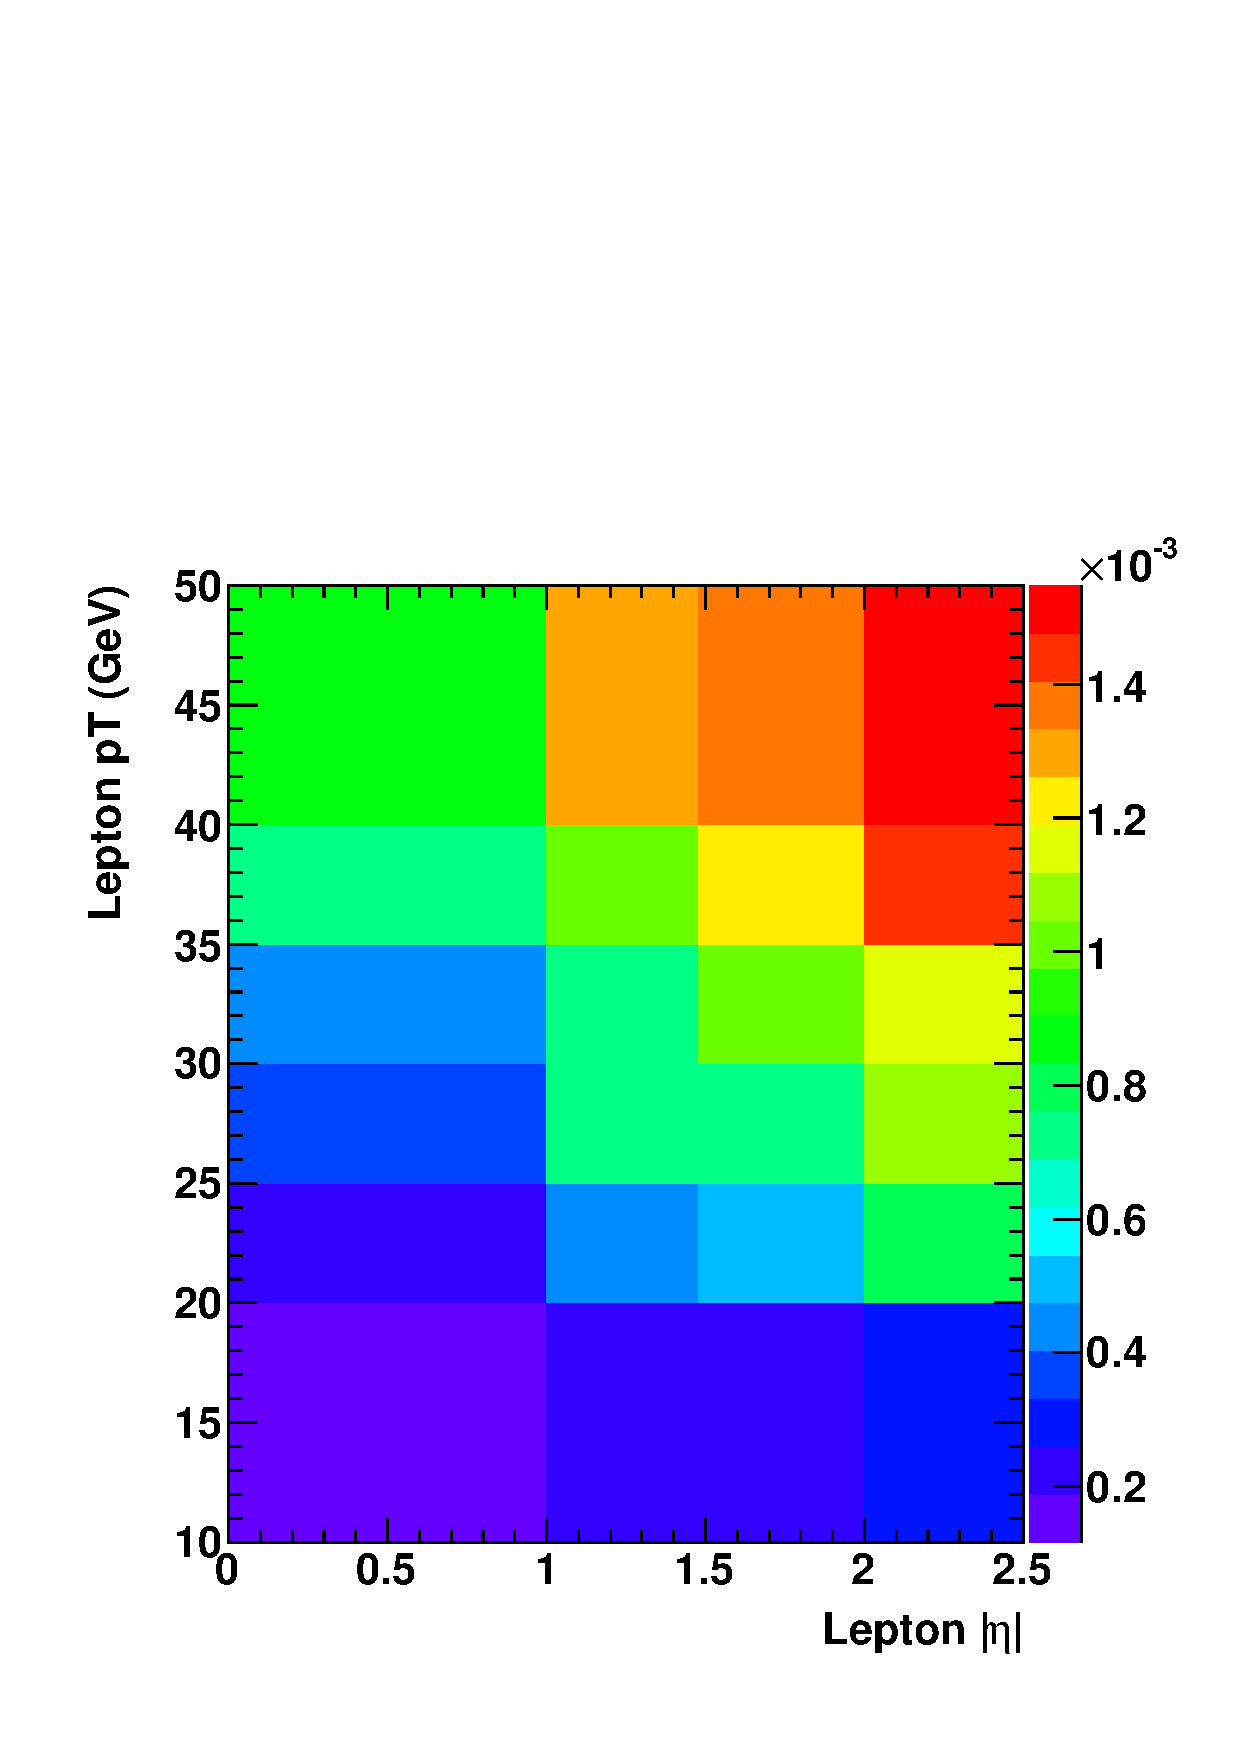
\includegraphics[width=0.4\textwidth]{figures/wjets_heleGenFR.pdf}                                            
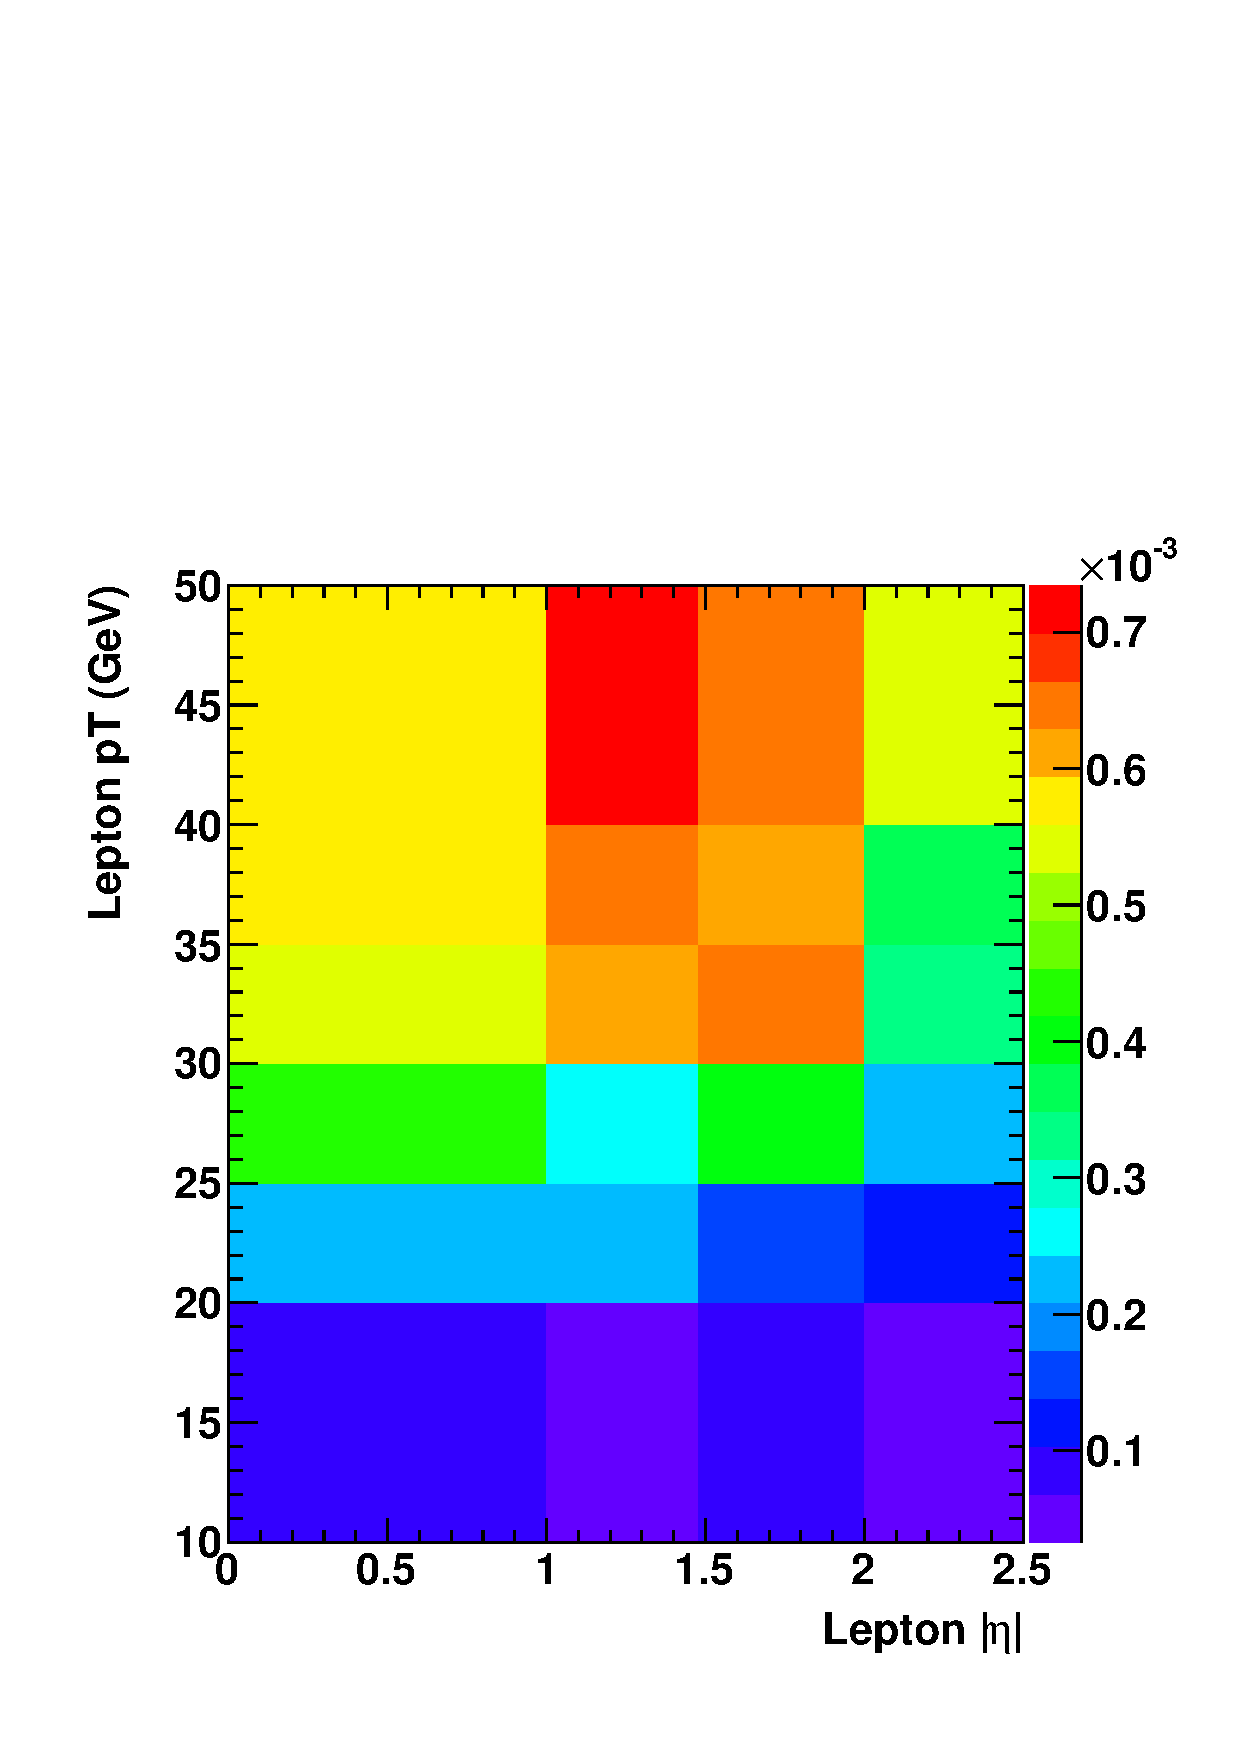
\includegraphics[width=0.4\textwidth]{figures/wjets_hmuGenFR.pdf}\\                                           
\caption{The probability for a parton to pass the electron (left) and muon (right)                            
fakeable object selections. }                                                                                 
\label{fig:lepgenfr}                                                                                          
\end{center}                                                                                                  
\end{figure}   

\begin{figure}[!htbp]                                                                                         
\begin{center}                                                                                                
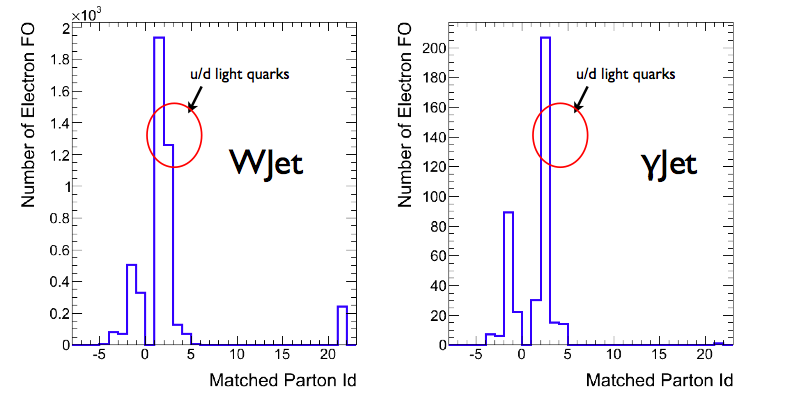
\includegraphics[width=0.8\textwidth]{figures/ElectronFakeOrigin.png}                                            
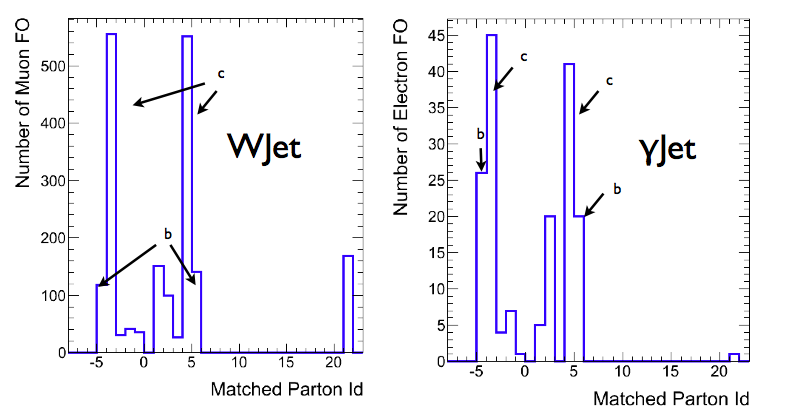
\includegraphics[width=0.8\textwidth]{figures/MuonFakeOrigin.png}\\                                           
\caption{ Origin of the electron and muon fakeable objects. The plot shows 
that electron fakes originate mostly from light quarks while muon fakes
are coming primarily from semi-leptonic heavy quark decays.}
\label{fig:fakeorigins}                                                                                          
\end{center}                                                                                                  
\end{figure}   


\begin{figure}[!htbp]                                                                                         
\begin{center}                                                                                                
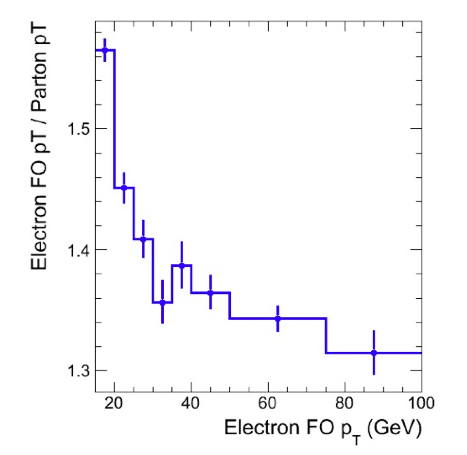
\includegraphics[width=0.4\textwidth]{figures/ElectronPtResponse.png}                                            
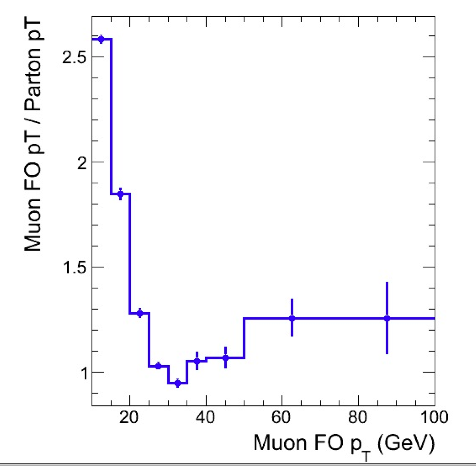
\includegraphics[width=0.4\textwidth]{figures/MuonPtResponse.png}\\                                           
\caption{Ratio of transverse momentum of a fakeable object and parton transverse momentum
for electron (left) and muons (right). }                                                                                 
\label{fig:ptresponse}                                                                                          
\end{center}                                                                                                  
\end{figure}   

\begin{figure}[!htbp]                                                                                         
\begin{center}                                                                                                
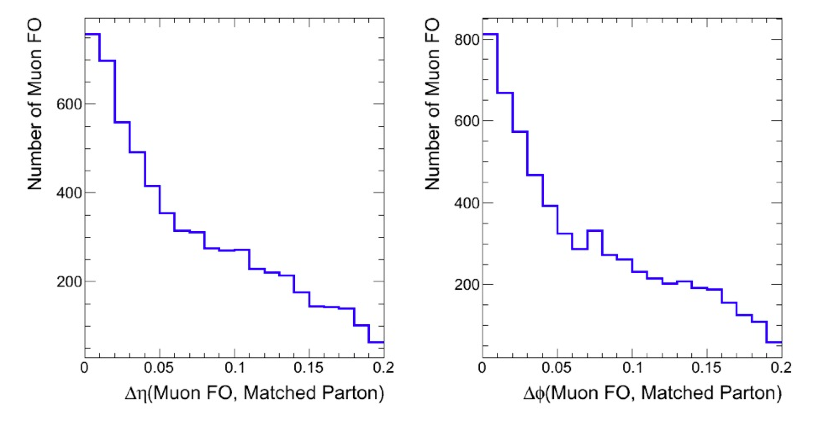
\includegraphics[width=0.8\textwidth]{figures/PartonLeptonDIrection.png}                                            
\caption{Distance in pseudo-rapidity (left) and azimuthal angle (right)
between generator level parton and reconstructed fakeable object.}                                                                                 
\label{fig:partonleptondirection}                                                                                          
\end{center}                                                                                                  
\end{figure}   

 
\subsection{$k_{T}$ Functions} 
In the leading order Matrix Element calculation there is no initial state radiation. The initial state partons 
collide head- on and the system has no transverse boost. To account for the transverse recoil and thus improve the performance 
of our discriminant on data, we integrate over the possible values of the system boost $K(kx,ky)$. The $K(kx,ky)$ model
is extracted from Monte Carlo for each process separately. Figure~\ref{fig:wwboost} shows the distribution of transverse boost for 
gluon fusion Higgs production and the non-resonant $W^{+}W^{-}$ processes

\begin{figure}[!htbp]                                                                                         
\begin{center}                                                                                                
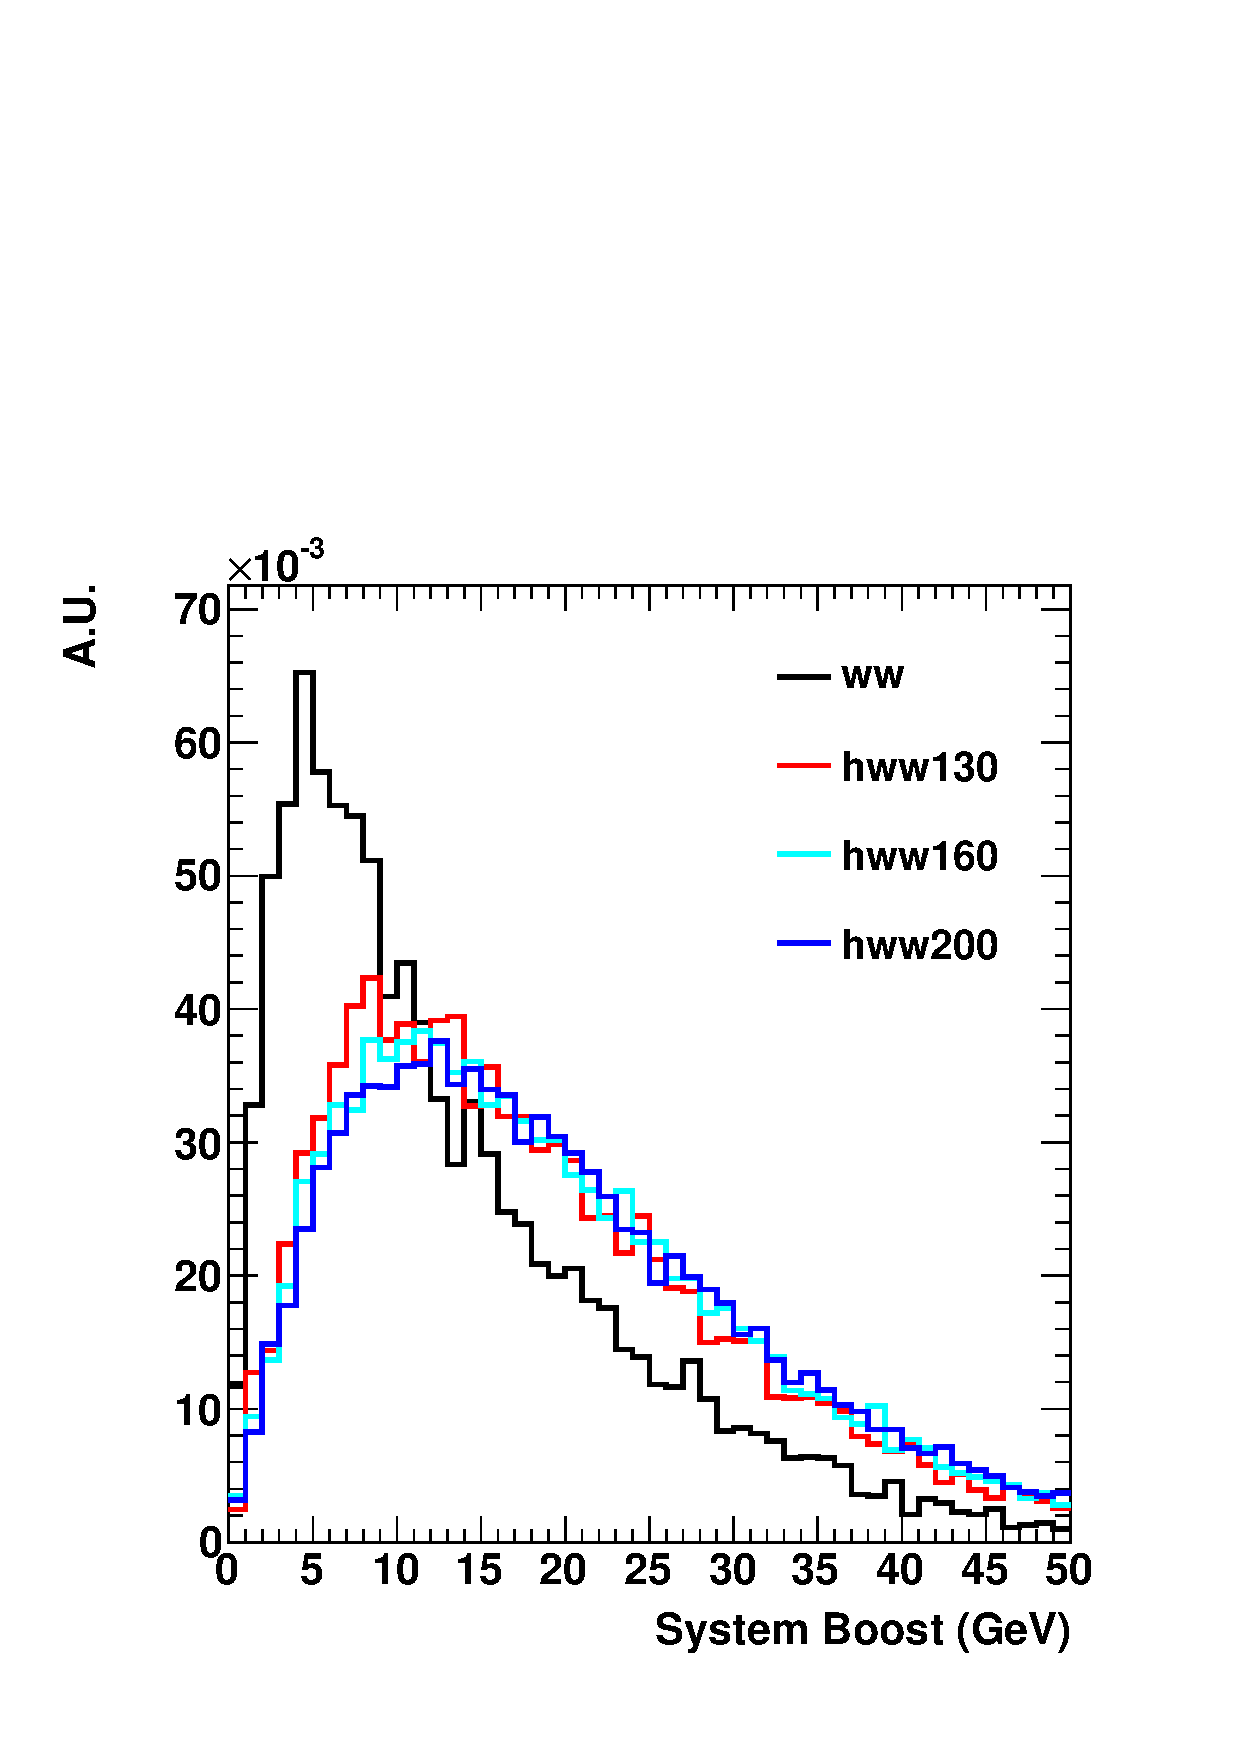
\includegraphics[width=0.5\textwidth]{figures/boost.pdf}                                                      
\caption{The transverse boost of the $WW$ system for $WW$ production and $H \rightarrow WW$ at 3 different Higgs masses.} 
\label{fig:wwboost}                                                                                           
\end{center}                                                                                                  
\end{figure}    

\subsection{Integration}
Evaluation of the differential cross section requires integration over missing kinematic information of an event, such 
as for example longitudinal components of neutrino momenta, as well as integration over allowed transverse momenta of the system.

We perfom integration using Monte Carlo technique, in which we generate values of unknown quantities based on a set of random numbers.
Monte Carlo calculations can be carried out using sets of random points picked from any arbitrary probability distribution. The choice 
of distribution obviously makes a difference to the efficiency of the method. In most cases, Monte Carlo calculations carried out 
using uniform probability distributions give very poor estimates of high-dimensional integrals and are not a useful method of approximation. 
Therefore, we employ algorithm of ``importance sampling'' into Monte Carlo integration. Instead of choosing points from a uniform distribution, 
they are chosen from a distribution which concentrates the points where the function being integrated is large, i.e.:
\begin{equation}
\label{eqn:ImpSampling}
I=\int_{x_{1}}^{x_{2}} f(x)dx = \int_{a}^{b} \frac{f(x)}{g(x)}dx,
\end{equation}
where the function $g(x)$ is chosen to be a reasonable approximation to $f(x)$. The integral can be calculated by choosing the random points 
from the probability distribution $g(x)$ and evaluating $f(x)/g(x)$ at these points.  Sampling from a non-uniform distribution for this function 
is more efficient than doing a crude Monte Carlo calculation without importance sampling.

Number of integration variables depends on the process for which differential cross-section is evaluated. For example, in the case of the
gluon fusion signal there are 4 missing components of the neutrino momenta:
\begin{equation}
\label{eqn:MissingInfo}
(\nu_{x}, \nu_{y}, \nu_{z}, \bar{\nu}_{z}).
\end{equation}
 These quantities in addition to the measured ones and with two components of the transverse boost $(k_{x},k_{y})$ fully define the system. However, 
integration using  $(\nu_{x}, \nu_{y}, \nu_{z}, \bar{\nu}_{z})$ set of variables is not efficient; due to the narrow Breit-Wigner width of 
the Higgs and $W$ bosons, most random points will be lying outside of the core of the cross-section function. To avoid this and improve 
efficiency of the integration we perform variable transformation $\nu_{x} \rightarrow M_{H}^{2}$ and $\nu_{y} \rightarrow M_{W}^{2}$ 
so that the set of integration variables becomes
$(M_{H}^{2}, M_{W}^{2}, \nu_{z}, \bar{\nu}_{z})$. A Jacobean corresponding to the transformation is calculated analytically and properly 
accounted for. The integration is then performed using importance sampling method, with neutrino components sampled by the exponential function and 
$M_{H}^{2}$ and $M_{W}^{2}$ using narrow Breit-Wigner. Similarly, for non-resonant $WW$ production, used set of integration variables is:
$(M_{W}^{2}, M_{W}^{2}, \nu_{z}, \bar{\nu}_{z})$. In the $W$+jet case, there is only one missing quantity $\nu_{z}$ which is sampled using 
exponentially falling function.

For each event we perform 100,000 integration steps. To verify that this is sufficient, for randomly selected events we calculate differential cross
sections using 500,000 integration steps and compare them to the ones obtained with 100,000. In vast majority of cases the difference was $< 1\%$ with
largest observed deviation of $\sim 5\%$. 


\section{Likelihood}
Event probabilities, calculated as described above, are used to construct 
a likelihood ratio discriminant, which we use in 1-dimensional template fit.  

The discriminator is defined as :
\begin{equation}
\label{eqn:LR}
LR = \frac { P_s} { P_s + \sum_i k_{bi} P_{bi}},
\end{equation}
where $k_{bi}$ are the relative ratio of expected contributions of each background
and satisfy $\sum k_{bi} =1$.
The calculation of $P_s$ is a function of Higgs mass so that likelihood ratio
shape depends on $m_H$. This is true for both signal and background templates of $LR$.

It is important to note that because LR distribution is calculated the same way for data, 
signal and backgrounds, the fact that we use LO Matrix Element and assume certain 
approximations in the analytic calculation may result in less than optimal sensitivity 
and but does not introduce biases.

\section{Systematics}
This section should be written. For now, all systematics are treated same way as in Note XXX.


\section{Results}

Figure~\ref{subfig:HWWXsec} shows differential gluon fusion cross section $d\sigma(H \rightarrow WW)/dx$ calculated
for gluon fusion signal and non-resonant $WW$ events. The distribution for signal events is shifted towards larger values of  $d\sigma(H \rightarrow WW)/dx$
compared to that for non-resonant $WW$, and has narrower width. Figure~\ref{subfig:HWWXsecvsdPhi} shows distribution of signal and non-resonant $WW$ events in  
$d\sigma(H \rightarrow WW)/dx$ vs $\Delta\phi$. The differential cross-section is correlated with $\Delta\phi$ and is on average decreasing with increasing 
azimuthal angle, which is expected from spin effects. Figure~\ref{subfig:Xsec_WWvsHWW} shows distributions of these events in $d\sigma(H \rightarrow WW)/dx$ 
vs $d\sigma(WW)/dx$ plane. One can see that while a certain level of separation can be achieved, there is a non-negligible overlapping region of phase space where
events from two processes are indistinguishable. Finally, figure~\ref{subfig:to be inserted} shows distributions of signal and $W$+jet 
events in $d\sigma(H \rightarrow WW)/dx$ vs $d\sigma(W+jet)/dx$ plane (this one needs to be made and inserted).

\begin{figure}[!hbtp]                                                                                         
\centering                                                                                                    
\subfigure[]{                                                                                                 
\centering                                                                                                    
\label{subfig:HWWXsec}                                                                                       
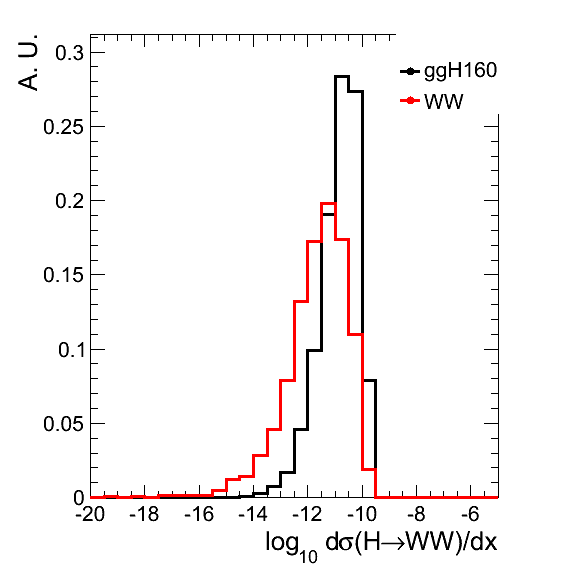
\includegraphics[width=.42\textwidth]{figures/HWWXsec.png}}                                                                                       
\subfigure[]{                                                                                                 
\centering                                                                                                    
\label{subfig:HWWXsecvsdPhi}                                                                                       
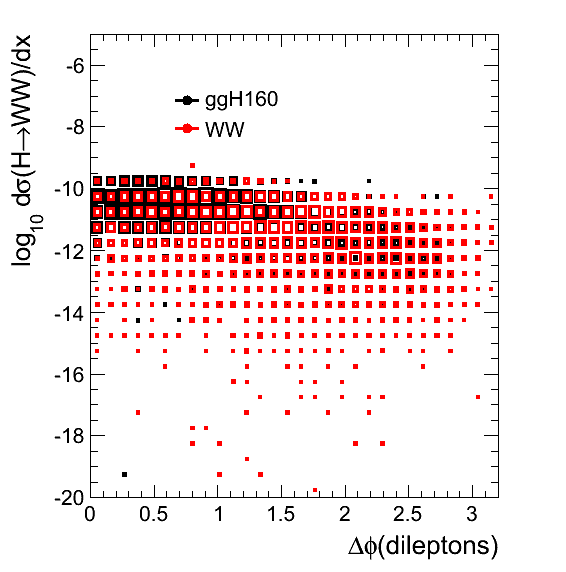
\includegraphics[width=.42\textwidth]{figures/HWWXsecvsdPhi.png}}                                            
\subfigure[]{                                                                                                 
\centering                                                                                                    
\label{subfig:Xsec_WWvsHWW}                                                                                       
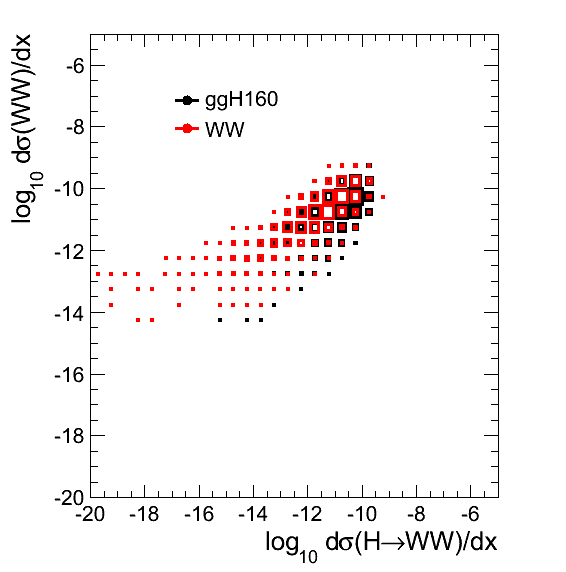
\includegraphics[width=.42\textwidth]{figures/Xsec_WWvsHWW.png}}\\                                            
\caption{The matrix element output LR distribution after $WW$ selection and $m_{ll}$ cut                      
for $m_H$=130 GeV \subref{subfig:lr_hm130}, $m_H$=160 GeV \subref{subfig:lr_hm160}, $m_H$=200 GeV 
\subref{subfig:lr_hm200} and $m_H$=300 GeV \subref{subfig:lr_hm300} in the 0-jet bin.}                                            
\label{fig:dXsecPlots}                                                                                          
\end{figure}                      

The effect of accounting for the transverse boost of the $WW$ system in the calculations of the 
differential cross-section is demonstrated in Figure~\ref{fig:kteffect}. In the absense of the boost, there is a tail in the Higgs event distribution 
 that have small values of $d\sigma(H \rightarrow WW)/dx$ and would be classified as background-like events. Accounting for the system boost removes the tail,
allowing for better signal and background discrimination. 

\begin{figure}[!hbtp]                                                                                         
\centering                                                                                                                                             
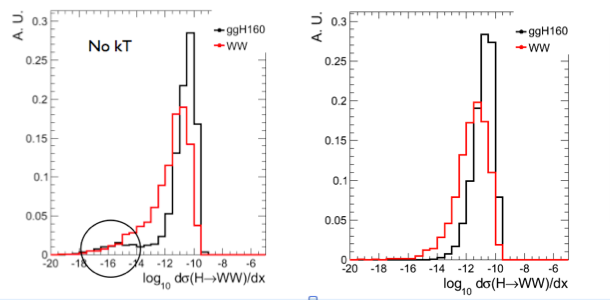
\includegraphics[width=.84\textwidth]{figures/SystemBoostEffect.png}\\                                            
\caption{The matrix element output LR distribution after $WW$ selection and $m_{ll}$ cut                      
for $m_H$=130 GeV \subref{subfig:lr_hm130}, $m_H$=160 GeV \subref{subfig:lr_hm160}, $m_H$=200 GeV 
\subref{subfig:lr_hm200} and $m_H$=300 GeV \subref{subfig:lr_hm300} in the 0-jet bin.}                                            
\label{fig:kteffect}                                                                                          
\end{figure}          


Figure~\ref{fig:lrstacks} shows the likelihood ratio distributions for $m_H$~=~130, 160, 200 and 300 GeV,               
corresponding to 1~fb$^{-1}$. Note that the majority of backgrounds peak near $LR~=~0$ while the signal peaks near $LR~=~1$.  
It has been noted earlier in the note that we apply dilepton invariant mass requirement prior to constructing likelihood ratio. 
Figure~\ref{fig:LR_noMll} shows likelihood ratio distribution for $M_{H}=160$ GeV mass hypothesis without the invariant mass requirements.
One can see from the peak at $LR~=~0$ that the Matrix Element method successfully identifies high invariant mass events as background like, so the cut
is not required. However, by applying the cut we loose less than $1\%$ of the signal and gain significantly in processing time.

\begin{figure}[!hbtp]                                                                                         
\centering                                                                                                    
\subfigure[]{                                                                                                 
\centering                                                                                                    
\label{subfig:lr_hm130}                                                                                       
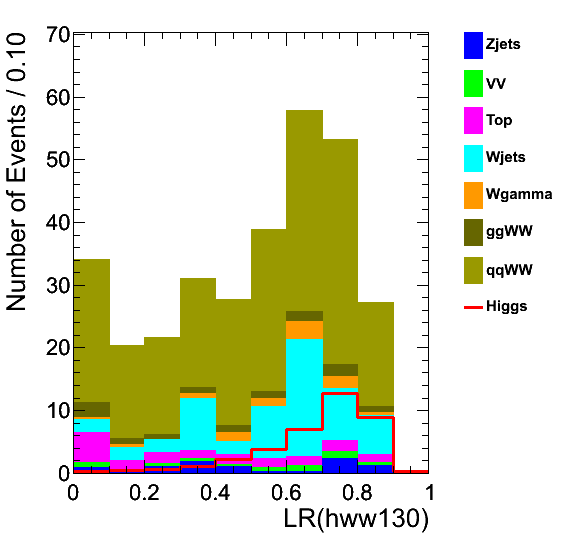
\includegraphics[width=.42\textwidth]{figures/hww130_LR.png}}                                                 
\subfigure[]{                                                                                                 
\centering                                                                                                    
\label{subfig:lr_hm160}                                                                                       
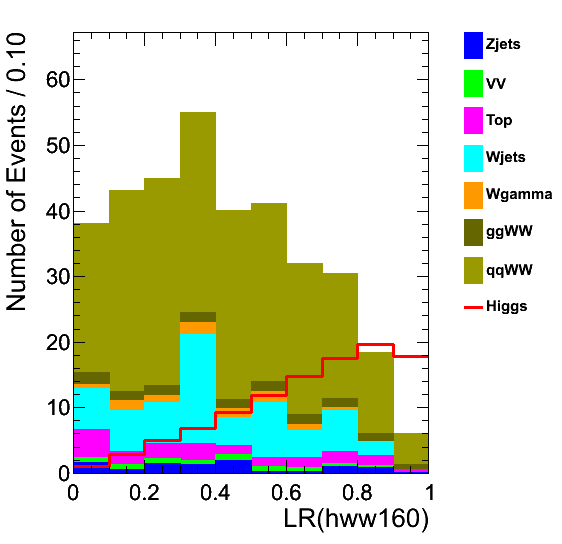
\includegraphics[width=.42\textwidth]{figures/hww160_LR.png}}                                                 
\subfigure[]{                                                                                                 
\centering                                                                                                    
\label{subfig:lr_hm200}                                                                                       
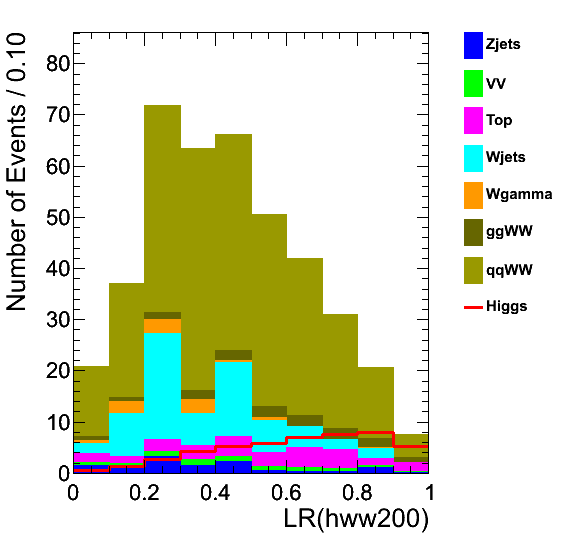
\includegraphics[width=.42\textwidth]{figures/hww200_LR.png}}
\subfigure[]{                                                                                                 
\centering                                                                                                    
\label{subfig:lr_hm300}                                                                                       
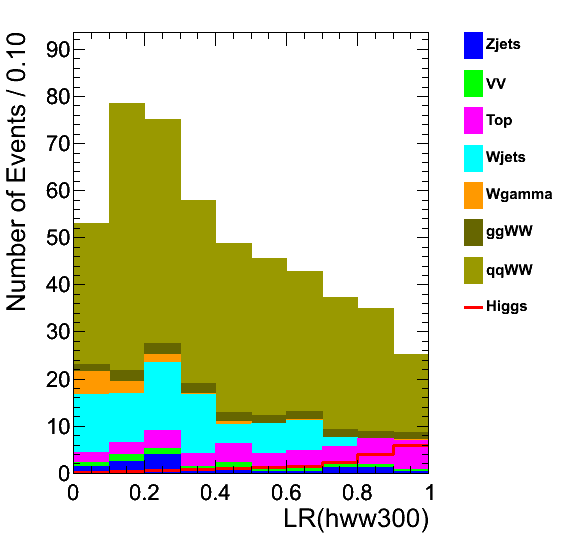
\includegraphics[width=.42\textwidth]{figures/hww300_LR.png}}\\                                              
\caption{The matrix element output LR distribution after $WW$ selection and $m_{ll}$ cut                      
for $m_H$=130 GeV \subref{subfig:lr_hm130}, $m_H$=160 GeV \subref{subfig:lr_hm160}, $m_H$=200 GeV 
\subref{subfig:lr_hm200} and $m_H$=300 GeV \subref{subfig:lr_hm300} in the 0-jet bin.}                                            
\label{fig:lrstacks}                                                                                          
\end{figure}                      


\begin{figure}[!hbtp]                                                                                         
\centering                                                                                                                                             
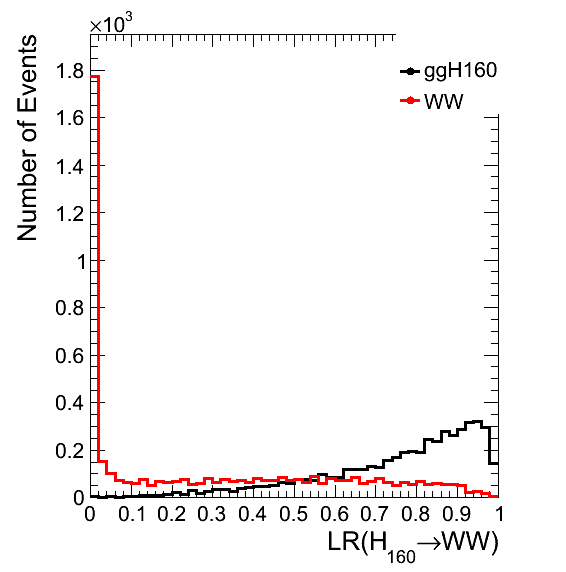
\includegraphics[width=.42\textwidth]{figures/LR_noMll.png}\\                                            
\caption{The matrix element output LR distribution after $WW$ selection but prior to $m_{ll}$ cut                      
for $m_H$=160 GeV}
\label{fig:LR_noMll}                                                                                          
\end{figure}       


We compute the upper limits using the shape of the LR to maximize the analysis sensitivity as described in 
Section~\ref{sec:results}. The expected upper limit at 95\%C.L as a function of $m_H$ using the LR are shown in 
Figure~\ref{fig:me_expected_1fb} comparing the corresponding results using the BDT output. 
The sensitivity performance of the matrix element method is consistent with the BDT based approach, with a 
slightly larger exclusion region. 

%%%%%%%%%%%%%%%%%%%%%%%%%%%%%%
\begin{figure}[!hbtp]
\centering
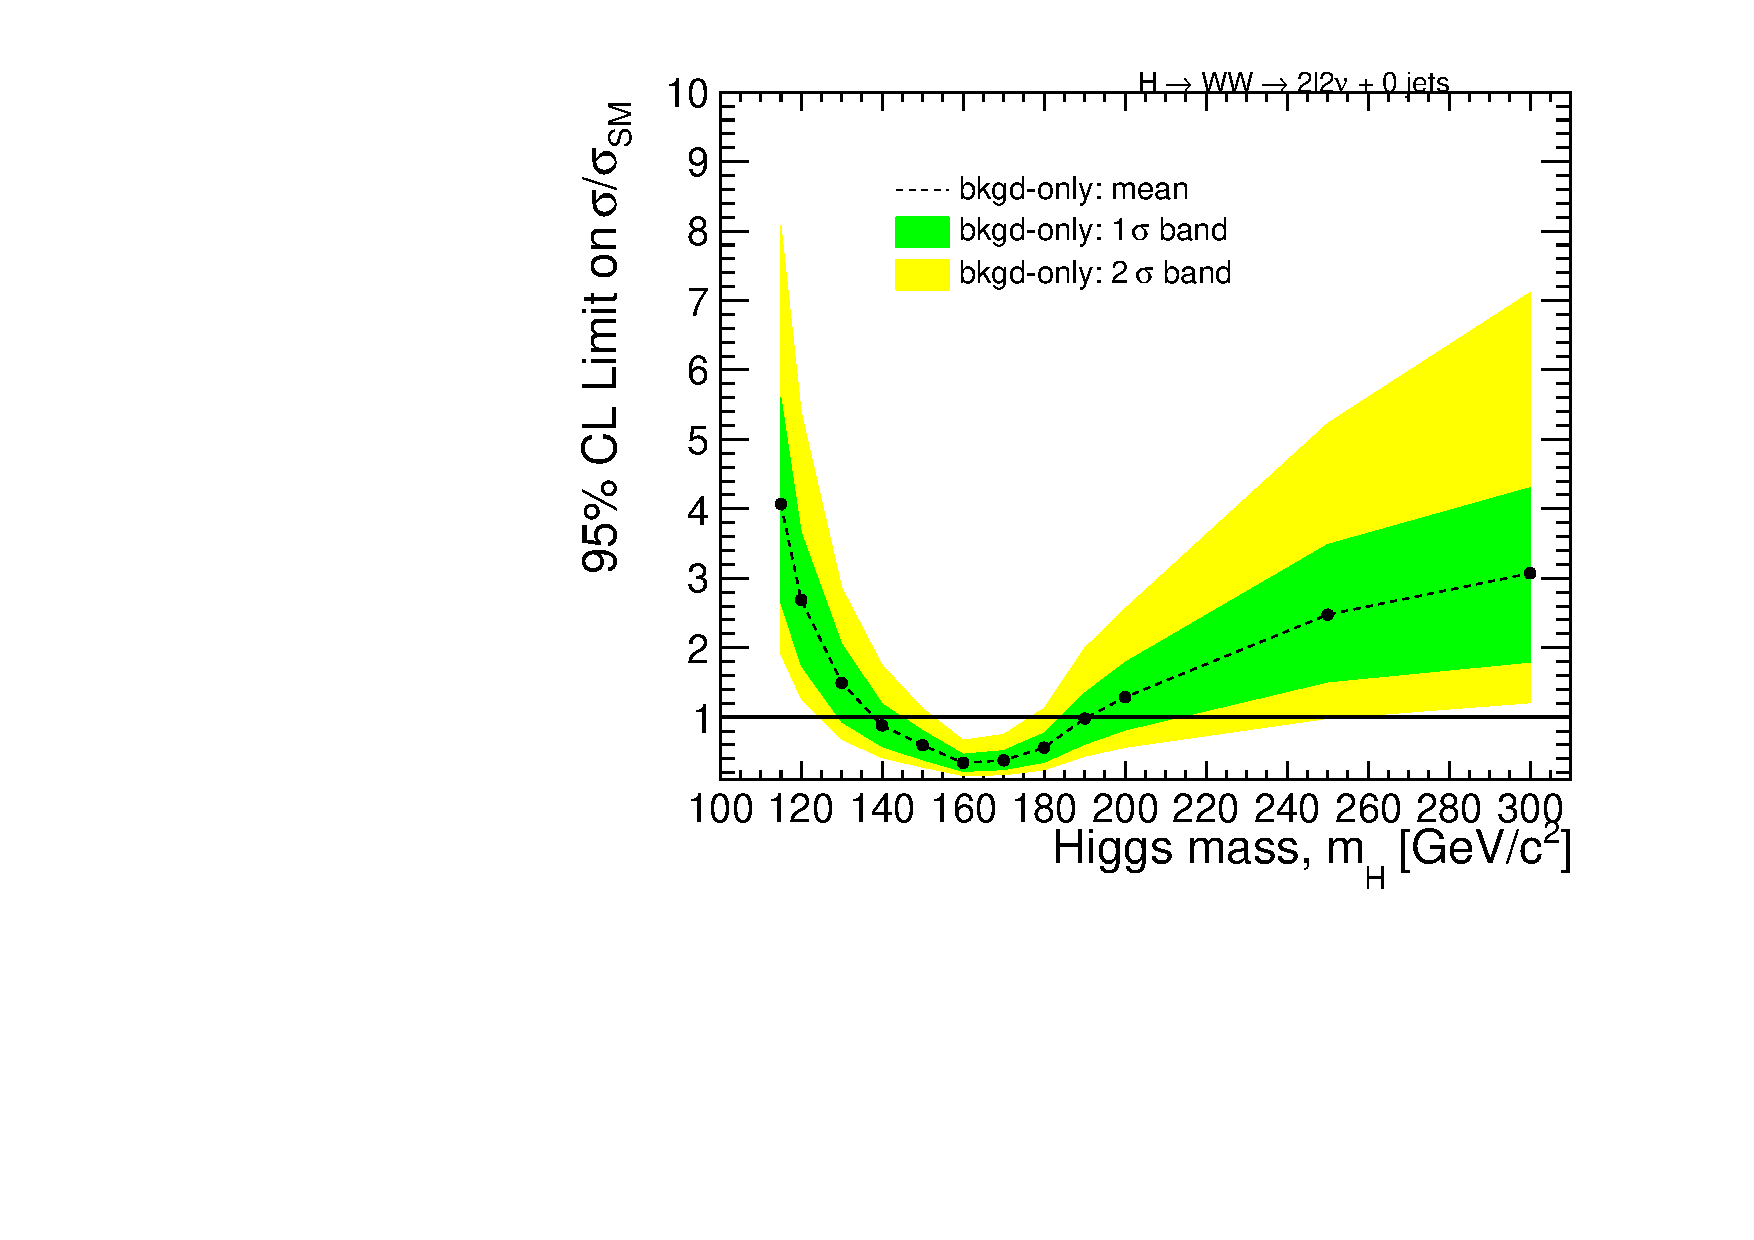
\includegraphics[width=.8\textwidth]{figures/limits_0j_1000pb_ME_shape.pdf}\\
\caption{ 
Multivariate shape analysis expected upper limits at 95$\%$ C.L. for 1~fb$^{-1}$ data using the 
matrix elemement output. } 
\label{fig:me_expected_1fb}
\end{figure}
%%%%%%%%%%%%%%%%%%%%%%%%%%%%%%

%%%%%%%%%%%%%%%%%%%%%%%%%%%%%%
\begin{table}[!hbtp]
\begin{center}
\begin{tabular}{c c c c c c c}
\hline\hline
 $m_H$ (GeV) & $-2\sigma$ & $-\sigma$ & mean & $+1\sigma$ & $+2\sigma$ \\
\hline
\multicolumn{6}{c} {Matrix Element Method} \\
\hline
115 & 1.90 &  2.64 &  4.07 &  5.60 & 8.08 \\
 120 & 1.27 &  1.75 &  2.69 &  3.66 & 5.39 \\
 130 & 0.68 &  0.93 &  1.49 &  2.05 & 2.86 \\
 140 & 0.42 &  0.58 &  0.88 &  1.19 & 1.75 \\
 150 & 0.28 &  0.39 &  0.60 &  0.81 & 1.12 \\
 160 & 0.16 &  0.22 &  0.34 &  0.47 & 0.67 \\
 170 & 0.17 &  0.24 &  0.38 &  0.52 & 0.75 \\
 180 & 0.24 &  0.35 &  0.56 &  0.77 & 1.13 \\
 190 & 0.44 &  0.61 &  0.98 &  1.35 & 1.99 \\
 200 & 0.57 &  0.81 &  1.29 &  1.79 & 2.56 \\
 250 & 0.98 &  1.51 &  2.48 &  3.49 & 5.23 \\
 300 & 1.21 &  1.79 &  3.07 &  4.30 & 7.11 \\
\end{tabular}
\end{center}
\caption{Multivariate shape analysis expected upper limits at 95$\%$ C.L. for 1~fb$^{-1}$ data using the 
matrix elemement output corresponding to Figure~\ref{fig:me_expected_1fb}.}
\label{tab:me_expected_1fb}
\end{table}


\end{document}